
\documentclass{beamer}
\usecolortheme{dove}
\setbeamertemplate{navigation symbols}{}
\usepackage{amsmath,amssymb,amsfonts,amsthm, multicol, subfigure, color}
\usepackage{bm}
\usepackage{graphicx}
\usepackage{tabularx}
\usepackage{booktabs}
\usepackage{hyperref}
\usepackage{pdfpages}
\usepackage{xcolor}
\definecolor{seagreen}{RGB}{46, 139, 87}
\def\independenT#1#2{\mathrel{\rlap{$#1#2$}\mkern2mu{#1#2}}}
\newcommand\indep{\protect\mathpalette{\protect\independenT}{\perp}}
\def\log{\text{log}}
\newcommand\logit{\text{logit}}
\newcommand\iid{\stackrel{\text{iid}}{\sim}}
\newcommand\E{\text{E}}
\newcommand\V{\text{V}}
\renewcommand\P{\text{P}}
\newcommand{\Cov}{\text{Cov}}
\newcommand{\Cor}{\text{Cor}}
\newcommand\doop{\text{do}}
\usepackage{stackrel}
\usepackage{tikz}
\usetikzlibrary{arrows,shapes.arrows,positioning,shapes,patterns,calc}
\newcommand\slideref[1]{\vskip .1cm \tiny \textcolor{gray}{{#1}}}
\newcommand\red[1]{\color{red}#1}
\newcommand\blue[1]{\color{blue}#1}
\newcommand\gray[1]{\color{gray}#1}
\newcommand\seagreen[1]{\color{seagreen}#1}
\newcommand\purple[1]{\color{purple}#1}
\newcommand\orange[1]{\color{orange}#1}
\newcommand\black[1]{\color{black}#1}
\newcommand\white[1]{\color{white}#1}
\newcommand\teal[1]{\color{teal}#1}
\newcommand\magenta[1]{\color{magenta}#1}
\newcommand\Fuchsia[1]{\color{Fuchsia}#1}
\newcommand\BlueGreen[1]{\color{BlueGreen}#1}
\newcommand\bblue[1]{\textcolor{blue}{\textbf{#1}}}
\newcommand\bred[1]{\textcolor{red}{\textbf{#1}}}
\newcommand\bgray[1]{\textcolor{gray}{\textbf{#1}}}
\newcommand\bgreen[1]{\textcolor{seagreen}{\textbf{#1}}}
\newcommand\bref[2]{\href{#1}{\color{blue}{#2}}}
\colorlet{lightgray}{gray!40}
\pgfdeclarelayer{bg}    % declare background layer for tikz
\pgfsetlayers{bg,main} % order layers for tikz
\newcommand\mycite[1]{\begin{scriptsize}\textcolor{darkgray}{(#1)}\end{scriptsize}}
\newcommand{\tcframe}{\frame{
%\small{
\only<1|handout:0>{\tableofcontents}
\only<2|handout:1>{\tableofcontents[currentsubsection]}}
%}
}

\usepackage[round]{natbib}
\bibliographystyle{humannat-mod}
\setbeamertemplate{enumerate items}[default]
\usepackage{mathtools}

\newcommand{\goalsframe}{\begin{frame}{Learning goals for today}
\begin{itemize}
    \item fundamental problem of causal inference
    \item potential outcomes
    \item recall mathematical concepts from probability
    \begin{itemize}
    \item random variables
    \item expectation
    \item conditional expectation
    \end{itemize}
\end{itemize} \vskip .2in
\end{frame}}

\title{Introduction to Computational Social Science}
\author{Ian Lundberg\footnote{Assistant Professor, Information Science, Cornell, \href{mailto:ilundberg@cornell.edu}{ilundberg@cornell.edu}}}
\date{SICSS UCLA\\24 June 2024}

\begin{document}

\maketitle

\begin{frame}

How would you define computational social science?

\end{frame}


\begin{frame}{How computing looked \textbf{in the 1950s}}
\begin{tikzpicture}[x = \textwidth, y = .8\textheight]
\node[anchor = north] (fig1) at (0,0) {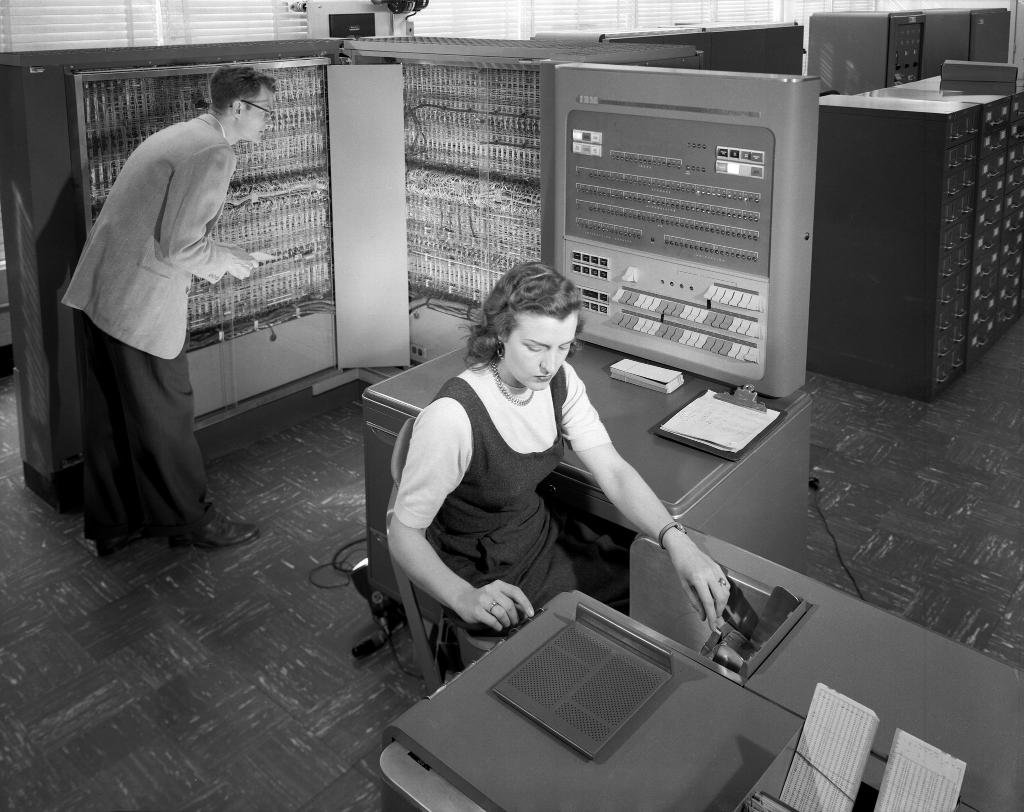
\includegraphics[width = .8\textwidth]{figures/punch_cards_nasa}};
\node[anchor = north west, font = \footnotesize] at (fig1.south west) {Source: \href{https://twitter.com/NASAhistory/status/1240971354003955712/photo/1}{NASA}};
\end{tikzpicture}
\end{frame}

\begin{frame}{How computing looked \textbf{in the 1980s}}
\begin{tikzpicture}[x = \textwidth, y = .8\textheight]
\node[anchor = north] (fig2) at (0,0) {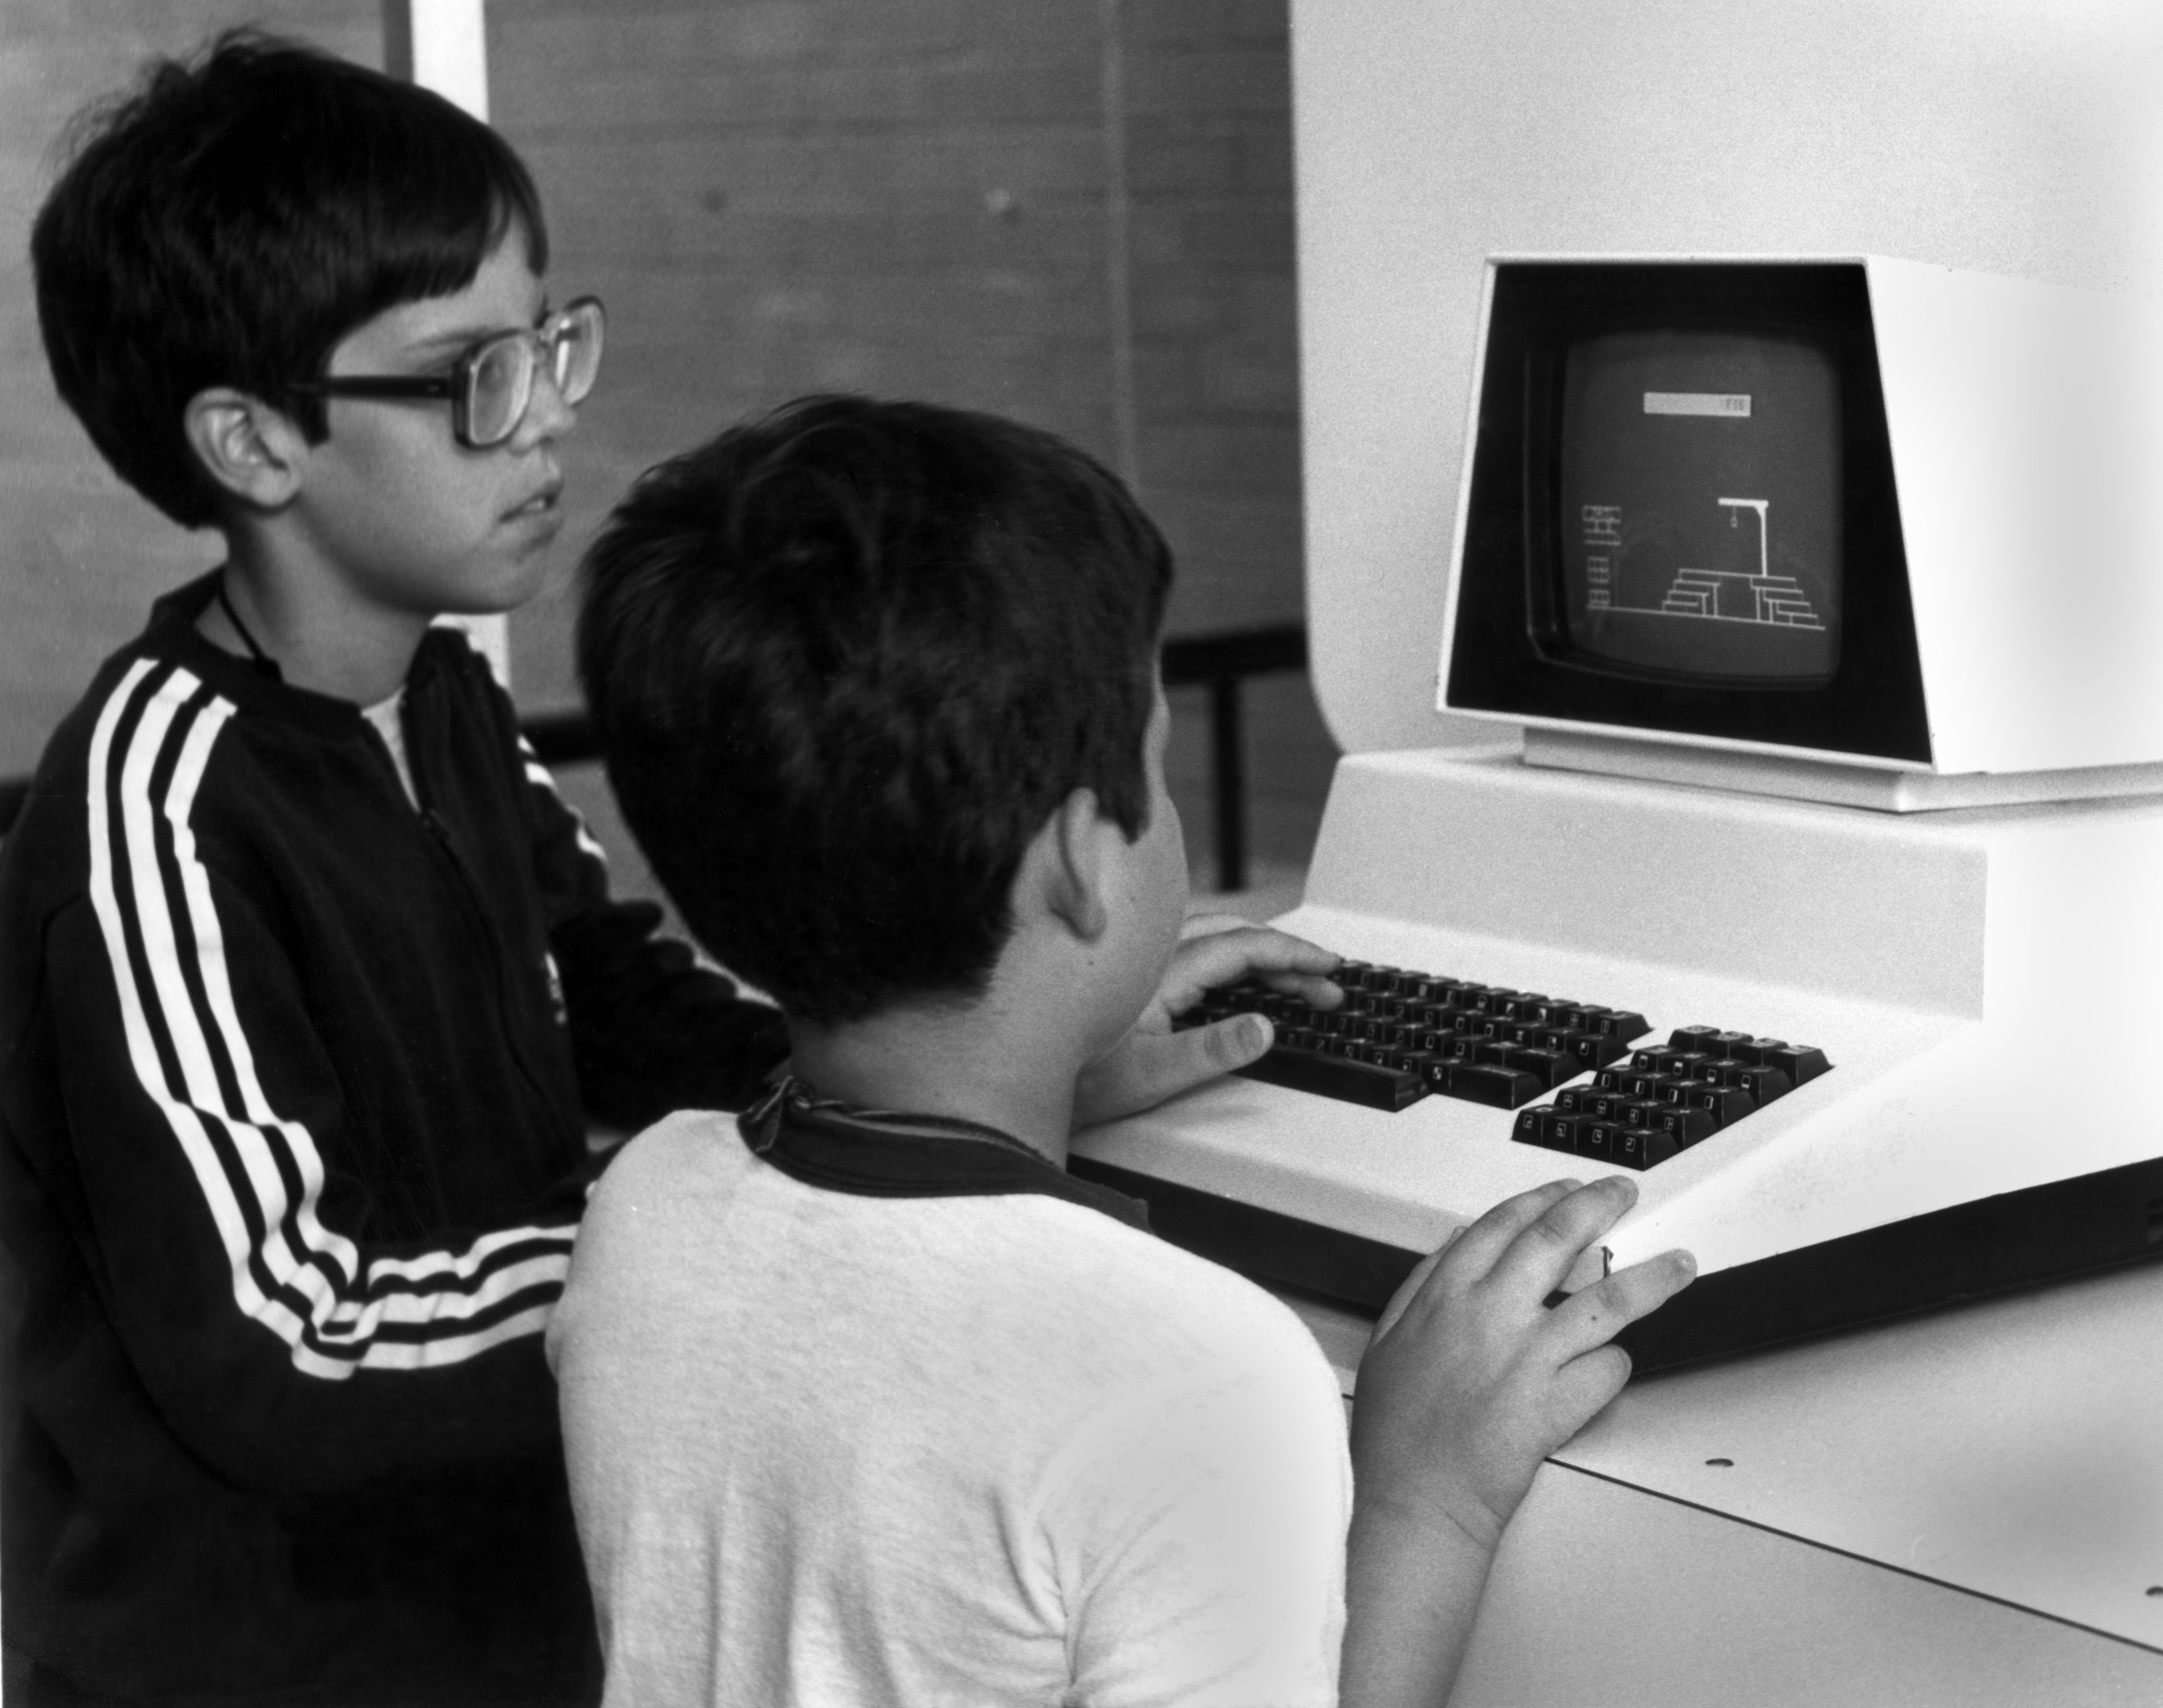
\includegraphics[width = .8\textwidth]{figures/pc}};
\node[anchor = north west, font = \footnotesize] at (fig2.south west) {Source: \href{https://commons.wikimedia.org/wiki/File:Commodore_PET_Exhibit_at_American_Museum_of_Science_and_Energy_Oak_Ridge_Tennessee.jpg}{Wikimedia}};
\end{tikzpicture}
\end{frame}

\begin{frame}{How computing looks \textbf{today}}
\begin{tikzpicture}[x = \textwidth, y = .8\textheight]
\node[anchor = north] (fig2) at (0,0) {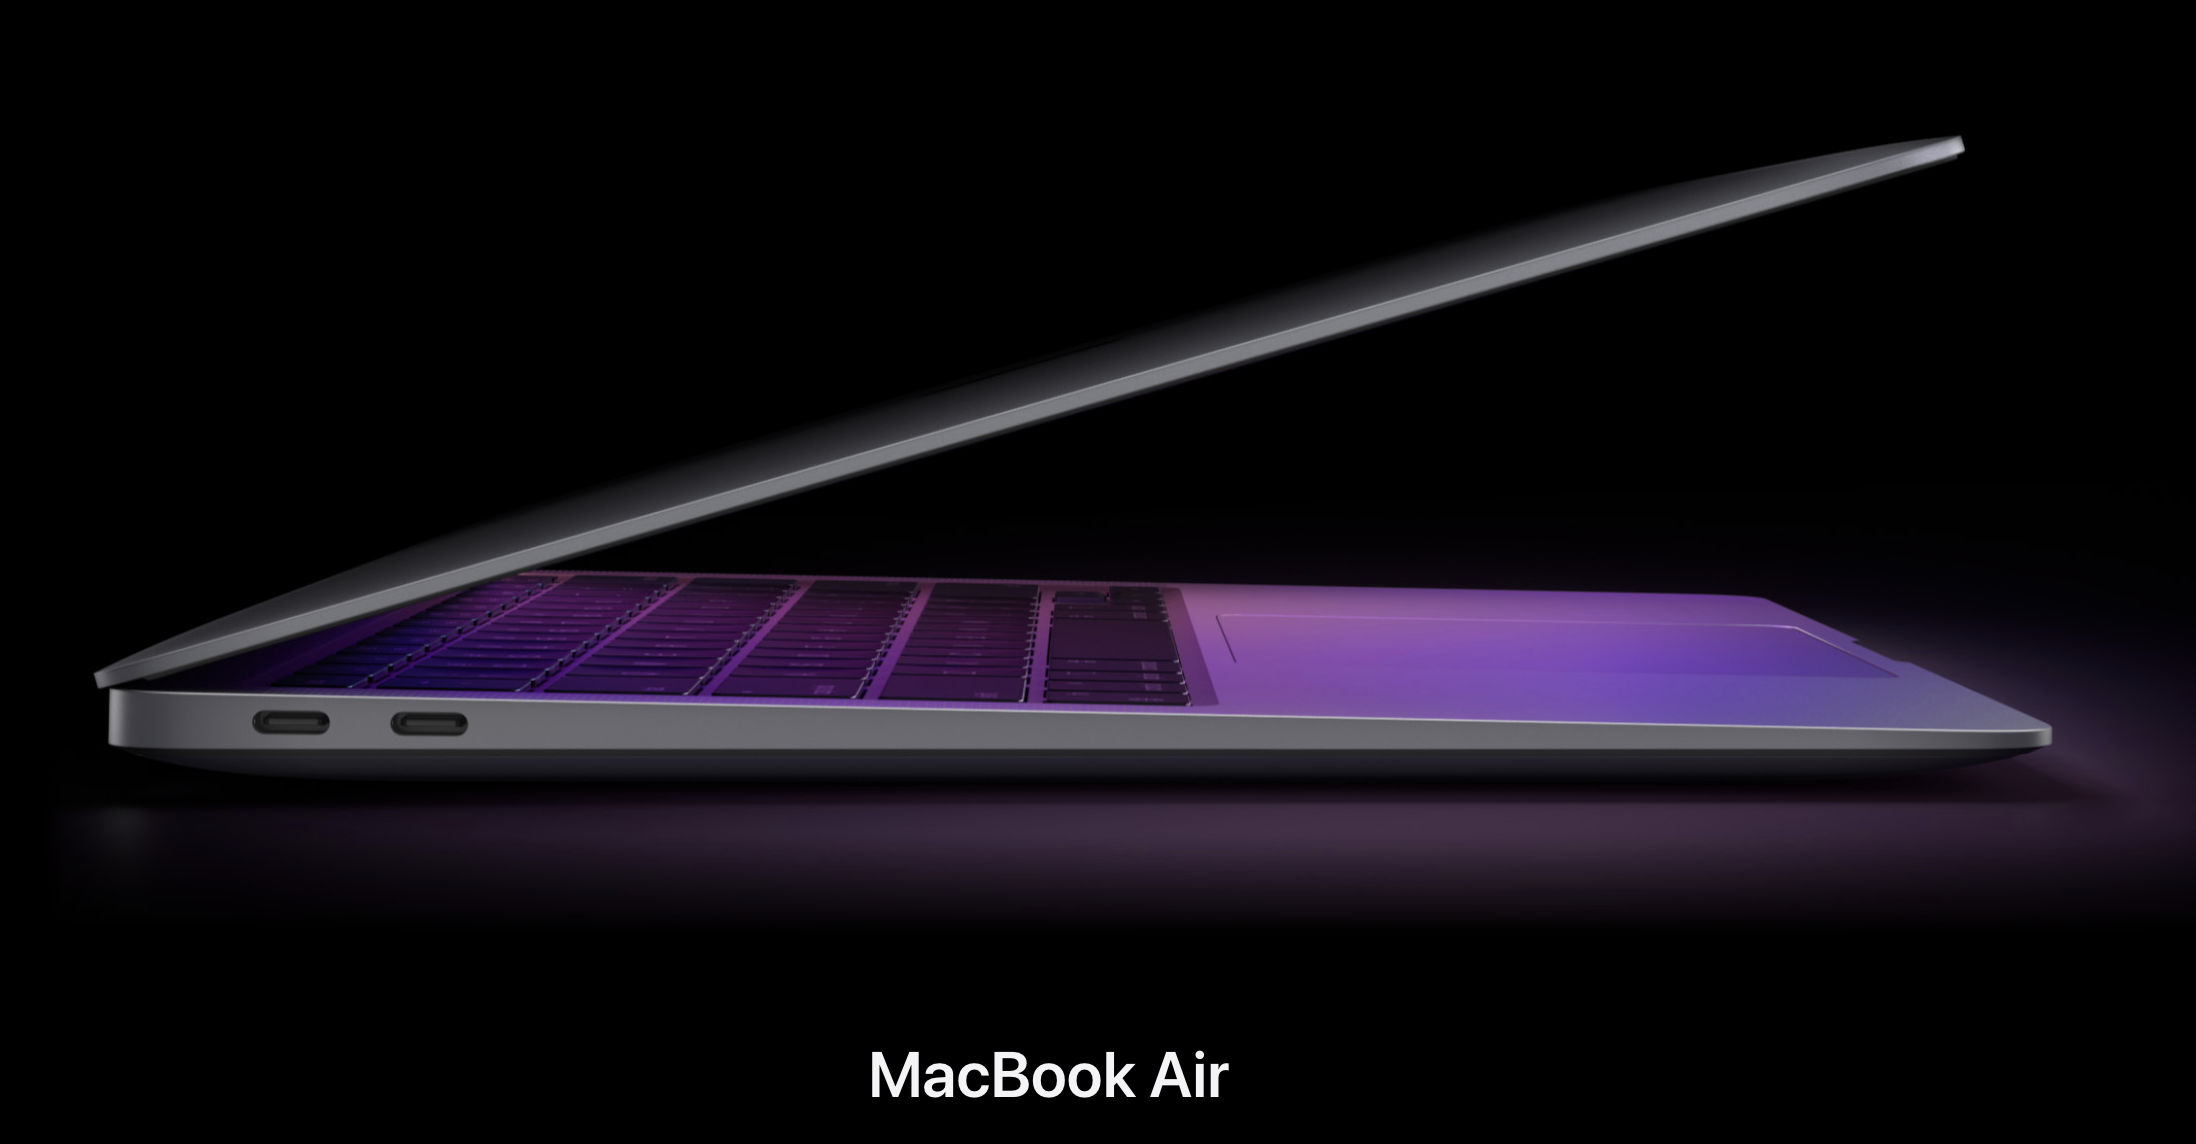
\includegraphics[width = \textwidth]{figures/macbook}};
\node[anchor = north west, font = \footnotesize] at (fig2.south west) {Source: \href{https://www.apple.com/macbook-air-m1/}{Apple}};
\end{tikzpicture}
\end{frame}

\begin{frame}{How computing looks \textbf{today}}
\begin{tikzpicture}[x = \textwidth, y = .8\textheight]
\node[anchor = north] (fig2a) at (0,0) {\includegraphics[width = .9\textwidth]{figures/chatGPT_sicss}};
\node[anchor = north west, font = \footnotesize] at (fig2a.south west) {Source: \href{https://chat.openai.com/chat}{OpenAI}};
\end{tikzpicture}
\end{frame}

\begin{frame}
%Computing has advanced rapidly since the 1960s \pause \vskip .4in
How might computing change the social sciences? \pause
\begin{itemize}[<+->]
\item new sources of data
\begin{itemize}
\item digital exhaust
\item text as data
\item online surveys
\item online experiments
\end{itemize}
\item new ways of working with data
\begin{itemize}
\item prediction with semi- and nonparametric models
\item simulation
\end{itemize}
\end{itemize}
\end{frame}

\begin{frame}
Whose ideas will help computational social science thrive? \vskip .2in \pause
Applied statisticians\pause,  computer scientists\pause,  survey methodologists\pause,  psychologists\pause,  demographers\pause,  sociologists\pause,  ethnographers\pause,  political scientists\pause,  economists\pause, policymakers\pause, corporate leaders\pause, community leaders\pause, ethics experts\pause, and more \vskip .2in \pause
Computational social science benefits from \textbf{everyone's ideas}
\end{frame}

\begin{frame}{Perspective that have shaped my thinking}
\small
\begin{itemize}
\item Athey, S. \& Imbens, G. (2018).  \bref{https://www.aeaweb.org/conference/cont-ed/2018-webcasts}{Machine Learning and Econometrics.} 2018 AEA Continuing Education Webcast. (Scroll down on website). See also review articles.
\item Efron, B., \& Hastie, T. (2016). \bref{https://hastie.su.domains/CASI/}{Computer age statistical inference: Algorithms, evidence, and data science.} Cambridge University Press.
\item Groves, R. M. (2011). \bref{https://doi.org/10.1093/poq/nfr057}{Three eras of survey research.} Public Opinion Quarterly, 75(5), 861-871.
%\item Athey, S., \& Imbens, G. W. (2019). Machine learning methods that economists should know about. Annual Review of Economics, 11, 685-725.
\item Salganik, M. J. (2019). \bref{https://www.bitbybitbook.com/}{Bit by bit: Social research in the digital age.} Princeton University Press.
\item Grimmer, J., Roberts, M. E., \& Stewart, B. M. (2022). \bref{https://press.princeton.edu/books/hardcover/9780691207544/text-as-data}{Text as data: A new framework for machine learning and the social sciences.} Princeton University Press.
\end{itemize}

\end{frame}

\end{document}
